\documentclass[11pt, a4paper, onecolumn, twoside, titlepage]{scrreprt}

% Header Datei einfügen
%%%%%%%%%%%%%%%%%%%%%%%%%%%%%%%%%%%%%%%%%
% Includings aller benötigten Packages!	%
%%%%%%%%%%%%%%%%%%%%%%%%%%%%%%%%%%%%%%%%%

% Akronyme
\usepackage{acronym}

% Algorithmen (i.d.R. nicht benötigt)
%\usepackage[plain,chapter]{algorithm}
%\usepackage{algpseudocode}

% Appendix
\usepackage[title]{appendix}

% Caption (Bildunterschriften)
\usepackage[
	format = plain,
	font = small,
	textformat = simple,
	justification = centering,
	labelfont = bf
]{caption}
\usepackage{subcaption}
\usepackage{chngcntr}
\usepackage[titles]{tocloft}

% Einstellungen der Seitenränder
\usepackage[
            left = 20mm,
			right = 30mm,
			top = 15mm,
			bottom = 20mm,
			headsep = 5mm,
   			footskip = 11mm,
			includeheadfoot]{geometry}

% Einrücken	der ersten Zeile eines Kapitels	
\usepackage{indentfirst}

% Enumarations
\usepackage{enumerate}
% Anpassbare Enumerates/Itemizes
\usepackage{enumitem}

% Farben und Grafiken
\usepackage[pdftex]{graphicx,color}
\usepackage{xcolor}
\usepackage{colortbl}

% Fonts
\usepackage{pifont}
\usepackage{lmodern}

% Hyperref - Cross-referencing
% https://www.namsu.de/Extra/pakete/Hyperref.html
% Komplette Doku: http://packages.oth-regensburg.de/ctan/macros/latex/contrib/hyperref/doc/manual.pdf
\usepackage[bookmarks = true,
			hypertexnames = true,
			pdfstartview = {FitH},
			colorlinks = true,
			linkcolor = black,
			citecolor = black,
			filecolor = black,
			urlcolor = black]{hyperref}

% Komascript Fix
\usepackage{scrhack}
\usepackage{listings}

% Kopf- und Fußzeilen
\usepackage[automark,
			headsepline,
			plainheadsepline,
			plainfootsepline]{scrlayer-scrpage}

% Mathematische Packages
\usepackage{amsmath,amsthm,amssymb}
\usepackage{mathtools}

% Mathematische Packages - beinhaltet Times New Roman als Font (Notwendig!)
\usepackage{mathptmx} 

% Paket zum Erstellen von Kommentaren 
%\usepackage{pdfcomment}

% Tabellen & Matrizen
\usepackage{tabularx}
\usepackage{calc}
\usepackage{array}

% Umlaute, Sprache, Unicode-Kodierung
\usepackage[english,ngerman]{babel}
\usepackage[utf8]{inputenc}
\usepackage[T1]{fontenc}

% URLs
\usepackage{url}

% Zeilennummerierung
% https://texblog.org/2012/02/08/adding-line-numbers-to-documents/
\usepackage{lineno}

% Zitation, Referenzen
\usepackage[square,sort,comma,numbers]{natbib}
\usepackage[german]{varioref}

% Anführungszeichen (Sollte nach "inputenc" importiert werden!)
\usepackage[autostyle=true,german=quotes]{csquotes}


%%%%%%%%%%%%%%%%%%%%%%%%%%%%%%%%%%%%%%%%%%%%%%%%%%
% Wichtig! Zuerst alle Settings personalisieren! %
%%%%%%%%%%%%%%%%%%%%%%%%%%%%%%%%%%%%%%%%%%%%%%%%%%
%%%%%%%%%%%%%%%%%%%%%%%%%%%%%%%%%%%%%%%%%%%%%%%%%%%%%%%%%%%
% Definition aller wichtigen Variablen und Einstellungen! %
%%%%%%%%%%%%%%%%%%%%%%%%%%%%%%%%%%%%%%%%%%%%%%%%%%%%%%%%%%%

% Angaben Student Allgemein

% Autor
\newcommand{\baauthor}{Sebastian Meissner}
% Matrikelnummer: Ohne führende 0 und ES, ohne Versionsnummer 
\newcommand{\bamatnum}{3084104}
% Titel der Bachelorarbeit
\newcommand{\batitle}{Anomalieerkennung in adaptiven Systemen mit Generativer KI}
% Fachsemester
\newcommand{\basem}{14}
% Ort (für Titelseite und eidesstattliche Erklärung)
\newcommand{\balocation}{Dorsten}

% Adresse Titelseite
\newcommand{\baadress}{
\baauthor \\
Wachtelstraße 74 \\
46282
\balocation \\
Matrikelnummer: \bamatnum
}

% Angaben Lehrstuhl (Betreuer, Gutachter, Zweitgutachter)

% Betreuer
\newcommand{\babetreuer}{Prof.\,Dr.\,Andreas Metzger}
% Erstgutachter
\newcommand{\bagutachter}{Prof.\,Dr.\,Andreas Metzger}
% Zweitgutachter
\newcommand{\bazgutachter}{Prof.\,Dr.\,ABC}


% Meta-Daten für das erzeugte PDF-File, Keywords bei Bedarf hinzufügen
\hypersetup{
	pdftitle    = {Seminararbeit \baauthor},
	pdfauthor   = {\baauthor},
	pdfsubject  = {\batitle},
	%pdfkeywords = {Stichwort1, Stichwort2, Stichwort3,....}
}

% Settings

% Abstand über Kapitelname verringern
\renewcommand*{\chapterheadstartvskip}{\vspace*{.5\baselineskip}}

% Numerierungstiefe
\setcounter{secnumdepth}{2}
\setcounter{tocdepth}{2}

% Pagestyle ,Header und Fußleisten

% Linien unter der Kopf- und über der Fußzeile
\KOMAoptions{
   headsepline = true,
   footsepline = true
}


% Vorherige Headereinstellungen überschreiben
\pagestyle{scrheadings}
\clearscrheadfoot

% Entfernt Nummerierung von Kapitelname in Kopfzeile
\renewcommand*{\chaptermarkformat}{}

% Aktueller Kapitelname wird ausgelesen und in der Kopfzeile links innen angezeigt
\automark[chapter]{chapter}
\ihead[\headmark]{\headmark}

% Links innen BA-Thema, Rechts außen BA-Thema Seitenzahl (1mm Abstand an beiden Seiten)
\ofoot*{\pagemark\hspace*{0.1mm}}

%%%%%%%%%%%%%%%%%%%%%%%%%%%%%%%%%%%%%%%%%%%%%%%%%%%%%%%%%%
% Wichtig! Sollte der Titel besonders lang sein und über %
% zwei Zeilen gehen: Variable \batitle ersetzen mit dem  %
% Themennamen und an geeigneter Stelle mit \\ einen      %
% manuellen Zeilenumbruch erzwingen.					 %
%%%%%%%%%%%%%%%%%%%%%%%%%%%%%%%%%%%%%%%%%%%%%%%%%%%%%%%%%%
\ifoot*{\hspace*{0.1mm}\footnotesize{\batitle}}

% Schriftgöße in Kopfleiste
\setkomafont{pageheadfoot}{\sffamily\small}
\renewcommand{\headfont}{\small}

% Schriftart zu Times New Roman
\setkomafont{disposition}{\bfseries}

% Schriftgröße für Chapter, Section, etc. ändern
\addtokomafont{chapter}{\LARGE}
\addtokomafont{section}{\Large}
\addtokomafont{subsection}{\large}
\addtokomafont{paragraph}{\itshape}

% Einrückung links bei jedem neuen Kapitel, Section, Subsection, Subsubsection
\setlength{\parindent}{0.5cm}

% Nummerierungsart der Bildunterschriften von Abbildungen und Tabellen
\makeatletter 
\counterwithout{figure}{chapter}
\counterwithout{table}{chapter}

\renewcommand{\thefigure}{\arabic{figure}} 
\renewcommand{\thetable}{\arabic{table}} 
\renewcommand{\cfttabpresnum}{\bfseries Tabelle } 
\renewcommand{\cftfigpresnum}{\bfseries Abbildung } 
\renewcommand{\cftfigaftersnum}{:} 
\renewcommand{\cfttabaftersnum}{:} 
\setlength{\cftfignumwidth}{2,5cm}                     
\setlength{\cfttabnumwidth}{2,0cm}                                           
\setlength{\cftfigindent}{0cm}                                                     
\setlength{\cfttabindent}{0cm} 
\makeatother


%%%%%%%%%%%%%%%%%%%%%%
% Nützliche Commands %
%%%%%%%%%%%%%%%%%%%%%%

% Leere Seite einfügen
\newcommand*{\blankpage}{%
  \clearpage\thispagestyle{empty}\null\newpage%
}

% Neuen Absatz einfügen mit 0.5cm Abstand nach links
% Nutzung:  ....abc def. \nAbsatz ghi jkl....
% Ergebnis: 
%			....abc def.
%			
%				ghi jkl....
\newcommand{\nAbsatz}{\newline\newline \noindent\hspace*{0.5cm}}

% Neuen Absatz beginnen am Anfang der neuen Zeile Abstand von 0.5cm nach links einfügen
\newcommand{\nEinrueck}{\noindent\hspace*{0.5cm}}

% z.B. mit Leerzeichen (kleiner und großer erster Buchstabe)
\newcommand{\stzB}{z.\,B. }
\newcommand{\stZB}{Z.\,B. }

% d.h. mit Leerzeichen (kleiner und großer erster Buchstabe)
\newcommand{\stdh}{d.\,h. }
\newcommand{\stDh}{D.\,h. }

% u.a. mit Leerzeichen (kleiner und großer erster Buchstabe)
\newcommand{\stua}{u.\,a. }
\newcommand{\stUa}{U.\,a. }

% Bild einfügen mit Bildunterschrift, Label für interne Verlinkung und Skalierung
% Nutzung: \mImage{caption}{label}{width-factor}{path}
% BSP: \mImage{Abbildung ABC}{abb:abc}{0.5}{uni-due-logo.png}
%
% Anmerkung: Die maximale Breite (bei Scalefaktor 1.0) ist die Breite des restlichen
% Textes. Bei mehrzeiliger Bildunterschrift wird der Text zentriert dargestellt.
\newcommand{\mImage}[4]{
	\begin{figure}[h!]
		\centering
		\includegraphics[width=\textwidth * \real{#3}]{./Bilder/#4}
		\captionsetup{width=\textwidth * \real{#3}}
		\caption{\label{#2}#1}
	\end{figure}    
}
\newcommand{\mImageCfg}[5]{
	\begin{figure}[#5]
		\centering
		\includegraphics[width=\textwidth * \real{#3}]{./Bilder/#4}
		\captionsetup{width=\textwidth * \real{#3}}
		\caption{\label{#2}#1}
	\end{figure}    
}

% Referenz auf Abbildung, referenzierbar anhand Label des zuvor definierten Bildcommands
% Zeigt: ".. Abbildung 2.x.x zeigt.."
% Nutzung: ".. \mImageRef{abb:uni-logo} zeigt.."
\newcommand{\mImageRef}[1]{\hyperref[#1]{Abbildung~\ref*{#1}}}

% Referenz auf Seitenzahl einer Abbildung, referenzierbar anhand Label des zuvor definierten Bildcommands
% Zeigt: "Auf Seite 12 sieht man..."
% Nutzung: "Auf \mPageRef{abb:uni-logo} sieht man..."
\newcommand{\mPageRef}[1]{\hyperref[#1]{Seite~\pageref*{#1}}}


% Beginn Dokument
\begin{document}

% Römische Seitenzahlen
\pagenumbering{Roman}

% Titelseite, leere Seite, Abstract
\thispagestyle{empty}
\newgeometry{left=25mm, right=35mm, top=25mm, bottom=30mm}

\begin{titlepage}
\begin{center}

\includegraphics[width=.8\textwidth]{Bilder/logo.pdf}

\vspace*{0.8cm}

\normalsize{Abteilung Software Engineering\\
Fakultät für Informatik\\
Universität Duisburg-Essen \\
\bigskip
Fachgebiet Adaptive Systeme\\
Prof. Dr. Andreas Metzger}

\vspace*{1.6cm}

\large{Seminararbeit}

\vspace*{0.6cm}

\LARGE{\textbf{\batitle}}

\vspace*{1.4cm}

\normalsize{Vorgelegt der Fakultät für Informatik\\
der Universität Duisburg-Essen (Campus Essen) von}

\vspace*{1.4cm}

\normalsize{\baadress}

\vspace*{1.0cm}

\small{\balocation, den \today}

\vspace*{1.5cm}

\normalsize{
\begin{tabular}{ll}
\textbf{Betreuung:} & \hspace*{1cm} \bagutachter\\
%\textbf{Zweitgutachter:} & \hspace*{1cm} \bazgutachter\\
\textbf{Studiengang:} & \hspace*{1cm} Software Engineering (B.\,Sc.)\\
\textbf{Semester:} & \hspace*{1cm} \basem
\end{tabular}
}

\end{center}
\end{titlepage}
\blankpage
\setcounter{page}{2}
\chapter*{Abstract}
\label{chapter:abstract}
Die zuverlässige Klassifikation von Anomalien in komplexen Systemen wirft eine zentrale Frage auf: Wie kann sichergestellt werden, dass ein als Anomalie identifizierter Datenpunkt tatsächlich eine Abweichung vom Normalverhalten darstellt, und nicht lediglich ein seltener, aber gültiger Ausdruck innerhalb des Systems? \\
Mit der zunehmenden Größe und Komplexität adaptiver Systeme stoßen klassische, meist lineare Verfahren zur Anomalieerkennung an ihre Grenzen. Besonders im Bereich von Big-Data-Architekturen, in denen Datenströme hochdimensional und dynamisch sind, gewinnt der Einsatz künstlicher Intelligenz zunehmend an Bedeutung.
Diese Seminararbeit beleuchtet den Einsatz generativer KI zur Anomalieerkennung in adaptiven Systemen. Anhand eines Fallbeispiels aus der aktuellen Fachliteratur wird gezeigt, wie generative adversariale Netzwerke zur Modellierung normaler Datenverteilungen genutzt werden können, um potenzielle Anomalien zu identifizieren. Ziel der Arbeit ist es, die theoretischen Grundlagen, Chancen und Herausforderungen dieser Technologie darzustellen und kritisch zu reflektieren, inwiefern generative KI einen Beitrag zur Weiterentwicklung klassischer Anomalieerkennungsverfahren leisten kann.


\renewcommand\thechapter{\Roman{chapter}}

% Inhaltsverzeichnis
\tableofcontents

%Abbildungsverzeichnis
\listoffigures
\addcontentsline{toc}{chapter}{Abbildungsverzeichnis}
\textbf{Abbildung 1:} CloudGEN Architektur – Seite 28
\nAbsatz
\textbf{Abbildung 2:} Modell Genauigkeit – Seite 29
\nAbsatz
\textbf{Abbildung 3:} Confusion Matrix – Seite 30
\nAbsatz
\textbf{Abbildung 5:} Bewertungsmetriken – Seite 31
\nAbsatz

\automark[chapter]{chapter}
\ihead[\headmark]{\headmark}

% Tabellenverzeichnis
\listoftables
\addcontentsline{toc}{chapter}{Tabellenverzeichnis}
\textbf{Abbildung 4:} Vergleich von Anomaieerkennungsmodellen für cloud Systeme. – Seite 30
\nAbsatz
\automark[chapter]{chapter}
\ihead[\headmark]{\headmark}

% Abkürzungsverzeichnis
% Nutzung siehe: https://www.namsu.de/Extra/pakete/Acronym.html
\chapter*{Abkürzungsverzeichnis}
\label{chapter:akronyme}
\begin{acronym}
	\acro{KI}{Künstliche Intelligenz}
	\acro{ChatGPT}{Chat Generative Pre-trained Transformer}
	\acro{ML}{Maschinelles Lernen}
    \acro{OCSVM}{One Class Support Vector Machines}
    \acro{RNN}{Rekurrente Neuronale Netze}
    \acro{GAN}{Gernerative Adversarialische Netze}
    \acro{ROC}{Receiver Operating Characteristic}
    \acro{LOF}{Local Outlier Factor}
    \acro{k-NN}{k-Nearest Neighbors}
    \acro{DBSCAN}{Density-Based Spatial Clustering of Applications with Noise}
    \acro{IQR}{Interquartilsabstand} 
    \acro{GMM}{Gaussian Mixture Models}
    \acro{LIME}{Local Interpretable Model-agnostic Explanations}
    \acro{SHAP}{Shapley Additive Explanations} 
    \acro{LSTM}{Long Short-Term Memory}
    \acro{CNN}{Convolutional Neural Networks}
\end{acronym}
\addcontentsline{toc}{chapter}{Abkürzungsverzeichnis}
\ihead[Abkürzungsverzeichnis]{}

% Arabische Seitenzahlen
\clearpage
\pagenumbering{arabic} 
\renewcommand\thechapter{\arabic{chapter}} 
\setcounter{chapter}{0}

% Reset Abbildungscounter
\setcounter{figure}{0}

%%%%%%%%%%%%%%%%%%%%%%%%%%%%%%%%%%%%%%%%%%%%%%%%%%%%
% Wichtig! Der Wechsel von arabischen zu römischen %
% Zahlen (und umgekehrt) erfordert immer ein       %
% manuelles Setzen der aktuellen Seitenzahl! 	   %
%%%%%%%%%%%%%%%%%%%%%%%%%%%%%%%%%%%%%%%%%%%%%%%%%%%%
\setcounter{page}{7}

\automark[chapter]{chapter}
\ihead[\headmark]{\headmark}

% Hauptteil , Einfügen aller Kapitel der Arbeit
\chapter{Einleitung und Grundlagen}
\label{ch:einl}
\section{Motivation}
Wie können wir sicher sein, dass Daten die in Echtzeit mithilfe von Generativer KI als Anomalie klassifiziert werden, wirklich Anomalien sind und keine Validen Daten. Durch eine stetige Zunahme von KI in Systemen und dabei immer komplexer und größer werdenden Datensystemen, mit Hinblick zu Big Data, wird die Erkennung von Anomalien ebenfalls schwieriger.\\ Fehlerhafte Anomalieerkennung kann jedoch schwerwiegende Folgen in Branchen wie dem \\ Gesundheitswesen, Finanzen oder der Cybersicherheit haben. Der Einsatz einer ausgereiften KI bietet nicht nur die Möglichkeit zuverlässig Anomalien in Echtzeit zu erkennen, sondern eventuell auch diese zu verstehen und vorhersagen zu können. Mein Interesse an diesem Thema wurde durch die Beobachtung geweckt , dass einige der fortschrittlichsten KI-Modelle wie Gemini, ChatGPT oder Microsoft Copilot selbst bei fehlerhaften Ergebnissen mit Überzeugung an deren Richtigkeit festhalten. Diese Eigenschaft wirft die Fragen auf, wie solche Modelle präzise für eine \\ Echtzeit-Anomalieerkennung genutzt werden können, während sie selbst noch anfällig für eigene Fehler sind. Mit dieser Arbeit möchte ich die Grenzen der Anomalieerkennung in adaptiven \\ Systemen mit bestehenden KI-Modellen analysieren und Ansätze zur Lösung dieser sowie \\ weiterer Probleme vertiefen. Eine verbesserte und präzisere Anomalieerkennung mithilfe \\generativer KI könnte Datenmissbrauch, Systemfehler und Betrug im Internet frühzeitig erkennen und so großen Schaden sowohl für Unternehmen als auch für Endnutzer verhindern. 

\label{sec:einl_motivation}
\section{Zielsetzung und Aufgabenstellung}
Das Ziel dieser Arbeit ist es, die Möglichkeiten der Anomalieerkennung im Bezug zu \\ adaptiven Systemen mit Hilfe von künstlicher Intelligenz zu analysieren und ihr Potenzial für \\ präzise Echtzeitanwendungen zu bewerten und zu  verbessern. Die Verbesserung dieser Systeme ist nicht nur für Unterschiedliche Branchen wie z.B.: der Cybersicherheit oder dem \\ Gesundheitswesen, sondern ebenfalls für jeden Endverbraucher im Internet. Dabei soll \\ insbesondere untersucht werden, wo verschiedene Ansätze der Anomalieerkennung von \\ unterschiedlichen generativen KI-Modellen ihre Stärken und Schwächen zu dem jetzigen Stand haben. Weitergehend möchte ich mögliche Lösungsansätze oder Optimierungsvorschläge zu den gegebenen Problemen und Schwächen in Echtzeit analysieren. Im Rahmen dieser Untersuchung werden folgende Forschungsfragen behandelt: \\ Welche generativen KI-Modelle eignen sich besonders für die Anomalieerkennung? \\ In welchen Szenarien zeigen sich Schwächen in der Echtzeitanwendung?\\ Welche datenbasierten Anforderungen müssen erfüllt sein, um generative Modelle erfolgreich \\ 
einzusetzen?\\ Die Analyse wird sich mit dem Vergleich generativer Modelle befassen, um ihre Eignung und \\ Herausforderungen bei praxisnahen Echtzeitanwendungen zu bewerten. Das Ziel ist es, die \\ aktuellen Grenzen und Probleme der Anomalieerkennung zu identifizieren und zu analysieren sowie konkrete Verbesserungsvorschläge zu bewerten, die die Leistungsfähigkeit und Zuverlässigkeit der Modelle steigern könnten.
\newpage
   
\label{sec:einl_zielsetzung}
\section{Aufbau der Arbeit}
Um das Thema dieser Seminararbeit klar und strukturiert darzustellen, gliedert sich die Arbeit in mehrere thematische Kapitel. Diese sind in einer aufeinander aufbauenden Logik geordnet, \\ beginnend mit grundlegenden Erläuterungen bis hin zu einer detaillierten Analyse und Diskussion der Ergebnisse. Nachfolgend wird der Aufbau im Detail erläutert.\\
\subsection*{1. Einleitung und Grundlagen}
\subsubsection*{1.1 Motivation: Persönliches Interesse und zentrale Fragestellung}
\subsubsection*{1.2 Zielsetzung und Aufgabenstellung: Ziele und Untersuchungsansätze}
\subsubsection*{1.3 Aufbau der Arbeit: Übersicht über die Struktur der Kapitel und deren Inhalte}
\subsubsection*{1.4 Grundlegende Begriffe}
\subsubsection*{1.5 Geplante Vorgehensweise: State of the Art}
\subsection*{2. Systematische Literaturrecherchen}
\subsection*{3. Anwendung anhand praktischer Beispiele}
\subsection*{4. Vor-/Nachteile und Grenzen} 
\subsection*{Literaturverzeichnis} 
\subsection*{Eigenständigkeitserklärung}

\label{sec:einl_aufbau}
\newpage





\section{Grundlegende Begriffe}
\label{sec:bsp_depth}


Ein adaptives System ist ein System, das über eine Möglichkeit verfügt, seine eigene \\ Leistung kontinuierlich in Bezug auf eine bestimmte Qualitätskennzahl oder optimale Bedingung zu überwachen und seine eigenen Parameter durch eine geschlossene Regelung so zu verändern, dass es sich diesem Optimum annähert\cite{AdaptiveSysteme}. Ein adaptives System basiert meistens auf den \\ MAPE-K Kreislauf. MAPE-K setzt sich aus verschiedenen Bestandteilen zusammen. Die erste Phase ist das Monitoring. Hierbei werden alle relevanten Informationen über das System \\ gesammelt. Es werden Metriken wie zum Beispiel: CPU- und Speicherauslastung, \\ Netzwerktraffic, Antwortzeiten oder spezialisierte Sensorwerte gesammelt. Dabei wird auch das Rauschen gefiltert und die unterschiedlichen Datenquellen werden in ein einheitliches Format \\ gebracht. Danach folgt der der Analyze Part. Hier werden die gesammelten Rohdaten aufbereitet und in Erkenntnisse übersetzt. Dies geschieht beispielsweise durch einen Schwellenwert-Check. Hier werden Engpässe, Trends und potenzielle Störzustände identifiziert. Die gefundenen \\Probleme werden nach Schweregrad und Häufigkeit priorisiert. Die dritte Phase ist der Plan. Die Plan-Phase entwirft konkrete Anpassungsstrategien basierend auf den Analyseergebnissen und der gespeicherten Wissensbasis. Dabei werden mehrere Aktionspläne generiert, die von \\ Konfigurationsänderungen bis hin zu einem Neustart führen können. Der letzte Schritt ist die Execute-Phase. In dem Execute-Schritt wird der ausgewählte Plan in das System umgesetzt.\\ Hierbei können Ressourcen hoch beziehungsweise runter skaliert werden oder auch \\Konfigurationsparameter angepasst werden.
Diese Punkte bilden oftmals den Grundsatz eines \\ adaptiven Systems und ergeben zusammen den MAPE-loop. Dieser loop wurde mit dem MAPE-K ansatz erweitert. Der Grundsatz wurde mit einer "Knowledge" Komponente erweitert. Diese \\ Komponente ist dabei keine weitere Phase die ausgeführt wird sondern viel mehr ein gemeinsamer Wissensspeicher, der vor jeder Phase Inputs wie Modelle, Regeln oder historische Daten liefert. Nach der Execute Phase fließen die Resultate direkt in Knowledge ein, um den nächsten Zyklus zu optimieren. Knowledge verbindet somit alle Phasen aber wird nicht als einzelne Phase separat am ende ausgeführt\cite{MAPEK}. 
\nAbsatz
Anomalieerkennung ist dabei ein entscheidendes Feld für die Datenanalyse in der \\ Monitoring-Phase. Es konzentriert sich auf die Identifizierung seltener, ungewöhnlicher oder \\ unerwarteter Ergebnissen oder Beobachtungen, die sich signifikant von der Mehrheit der Daten \\ unterscheidet. Solche Abweichungen, auch als Ausreißer bezeichnet, können wichtige \\ Informationen liefern, etwa über Cyberangriffe, Systemausfälle, Betrug oder Fehler. Durch die steigende Menge von komplexeren Daten und Systemen in verschiedenen Bereichen ist die \\ manuelle Anomalieerkennung unpraktisch geworden. Dies führte zu einer Automatisierung der \\ Erkennungsprozesse durch das Einführen von KI und ML Verfahren. Ein Vorteil von KI-gestützter Anomalieerkennung im Gegensatz zu der manuellen ist eine dynamische Anpassung an neuen Datenmustern. KI-Modelle können ebenfalls feinere Unregelmäßigkeiten frühzeitig erkennen und sich mit wachsender Anzahl an Trainingsdaten verbessern\cite{LOF}. \nAbsatz
Eine Anomalie wird als ein Muster in Daten definiert, das nicht einer klar definierten \\ Vorstellung von normalem Verhalten entspricht. In einem Datensatz existieren oft normale \\ Regionen, in denen sich die Mehrheit der Datenpunkte befindet. Beobachtungen, die sich \\ signifikant von diesen normalen Regionen entfernen, gelten als Anomalien.
Solche Anomalien können durch verschiedene Faktoren verursacht werden, darunter betrügerische Aktivitäten \\ (z. B. Kreditkartenbetrug), Cyberangriffe, Systemausfälle oder andere außergewöhnliche \\ Ereignisse. \newpage Die Erkennung von Anomalien ist besonders relevant, da sie in vielen Fällen von Interesse für Analysten sind – sei es zur Sicherheitsüberwachung, Betrugsprävention oder Fehlermeldung.
Die Anomalieerkennung unterscheidet sich von verwandten Konzepten wie der Rauschentfernung und der Rauschakkommodation. Während Rauschentfernung darauf abzielt, störende und irrelevante Daten vor einer Analyse zu beseitigen, befasst sich die Rauschakkommodation damit, statistische Modelle gegen solche unerwünschten Abweichungen zu immunisieren.
Ein weiteres verwandtes Konzept ist die Neuheitenerkennung, die sich mit der Identifikation neuer oder zuvor unbekannter Muster befasst. Im Gegensatz zur Anomalieerkennung werden neuartige Muster nach ihrer Identifikation oft in die normale Modellierung integriert. Dennoch gibt es Überschneidungen zwischen den Ansätzen, sodass Methoden der Neuheitenerkennung häufig für die Anomalieerkennung \\ genutzt werden und umgekehrt\cite{LOF}.
  \nAbsatz
Fortschrittliche Anomalieerkennungssysteme können drei Haupttypen von Anomalien \\ identifizieren: Punkt-, kontextbezogene und kollektive Anomalien. Das Verständnis dieser \\ Unterscheidungen ist entscheidend für die Auswahl geeigneter Erkennungsmethoden und die \\ Interpretation von Ergebnissen\cite{LOF}. 
\begin{itemize} \item \textbf{Punktanomalien:} \end{itemize} Wenn ein einzelner Datenpunkt im Vergleich zum restlichen Datensatz als ungewöhnlich \\ angesehen wird, spricht man von einer Punktanomalie\cite{LOF}. Dies ist die einfachste Art der Anomalie und steht im Mittelpunkt der meisten Forschungsarbeiten zur Anomalieerkennung.

\begin{itemize} \item \textbf{Kontextbezogene Anomalien:} \end{itemize} Wenn eine Dateninstanz in einem bestimmten Kontext als anomal betrachtet wird, jedoch nicht allgemein, spricht man von einer kontextuellen Anomalie (auch bedingte Anomalie bezeichnet). Der Kontext ergibt sich aus der Struktur des Datensatzes und muss als Teil der Problemformulierung spezifiziert werden\cite{LOF}. Dinge wie Zeit, Umgebung oder andere relevante Variablen spielen hier eine Rolle. \\
\begin{itemize} \item \textbf{Kollektive Anomalien:} \end{itemize} Wenn eine Gruppe zusammenhängender Dateninstanzen im Vergleich zum gesamten Datensatz als ungewöhnlich erscheint, spricht man von einer kollektiven Anomalie. Dabei zeigen die \\einzelnen Datenpunkte meist keine auffälligen Abweichungen, erst ihr gemeinsames Auftreten enthüllt das abnorme Muster\cite{LOF}. \nAbsatz
Es gibt 4 Fehlerkategorien: \\
\begin{itemize} \item \textbf{1. True Positive (Richtig-Positiv):} \end{itemize}
Dies beschreibt einen Fall, bei dem ein Modell ein Ereignis korrekt als vorhanden erkennt. Ein True Positive bedeutet, dass das Modell sowohl in der Identifikation als auch in der Klassifikation richtig liegt.
True Positives sind wünschenswert, da sie zeigen, dass das Modell in der Lage ist, relevante Ereignisse oder Muster effektiv zu erkennen\cite{Fehlerkategorie}.

\\
\begin{itemize} \item \textbf{2. True Negative (Richtig-Negativ):} \end{itemize}
Bei einem True Negative erkennt das Modell korrekt, dass ein Ereignis nicht vorhanden ist. Es handelt sich um eine korrekte Ablehnung, wenn keine Abweichung oder Besonderheit vorliegt. True Negatives sind wichtig, um unnötige Alarme oder Fehlklassifikationen zu vermeiden. Sie tragen dazu bei, dass das Modell nicht übermäßig sensibel reagiert\cite{Fehlerkategorie}.

\\
\begin{itemize} \item \textbf{3. False Positive (Falsch-Positiv):} \end{itemize}
Ein False Positive tritt auf, wenn ein Modell ein Ereignis fälschlicherweise als vorhanden erkennt, obwohl es nicht existiert. Diese Art von Fehler kann zu übermäßigen oder unnötigen Aktionen führen. Sie zeigen, dass das Modell möglicherweise zu sensibel eingestellt ist\cite{Fehlerkategorie}.

\\
\begin{itemize} \item \textbf{4. False Negative (Falsch-Negativ):} \end{itemize}
Ein False Negative tritt auf, wenn das Modell ein tatsächliches Ereignis übersieht und \\ fälschlicherweise als nicht vorhanden einstuft. Diese Fehlerart ist oft besonders kritisch, da sie dazu führen kann, dass wichtige Probleme unentdeckt bleiben. False Negatives sind gefährlich da sie potenziell schwerwiegende Konsequenzen haben können. Dies kann auf eine unzureichende Sensibilität des Modells hinweisen\cite{Fehlerkategorie}.
\nAbsatz
Anomalieerkennungstechniken lassen sich grob in statistische Methoden, Methoden des maschinellen Lernens und Deep-Learning-Methoden einteilen. Die Wahl der Methode hängt von der Art der Daten, der Art der erwarteten Anomalien und der Verfügbarkeit von gekennzeichneten Daten ab\cite{LOF}.  \\
\begin{itemize} \item \textbf{Statistische Methoden:} \end{itemize} Das zentrale Prinzip der statistischen Anomalieerkennung besagt, dass eine Beobachtung als \\ Anomalie gilt, wenn sie teilweise oder vollständig außerhalb des durch ein angenommenes \\ stochastisches Modell definierten Verhaltensbereichs liegt. Es wird davon ausgegangen, dass \\ normale Datenpunkte in den Regionen von hoher Wahrscheinlichkeit des Modells vorkommen, während Abweichungen in den Bereichen geringer Wahrscheinlichkeit zu finden sind.\\
Die Vorgehensweise statistischer Methoden besteht darin, zunächst ein Modell zu entwickeln, dass das typische Verhalten der Daten repräsentiert. Anschließend kommt ein statistischer \\ Inferenztest zum Einsatz, um zu bestimmen, ob eine neue Beobachtung mit dem erstellten Modell übereinstimmt. Beobachtungen, die nach diesem Test nur mit sehr geringer Wahrscheinlichkeit aus dem Modell stammen könnten, werden als Anomalien identifiziert.\\
Zur Modellanpassung werden sowohl parametrische als auch nichtparametrische Ansätze \\ verwendet. Parametrische Methoden nehmen an, dass die zugrunde liegende Verteilungsform \\ bereits bekannt ist und schätzen anhand der vorliegenden Daten die entsprechenden Parameter. Im Gegensatz dazu setzen nichtparametrische Verfahren üblicherweise keine konkreten Annahmen über die Verteilungsstruktur voraus. Anschließend erfolgt eine detaillierte Betrachtung beider \\ Ansätze zur Anomalieerkennung. Dieser Ansatz dient meistens in dynamischen \\ adaptiven Systemen oft als Basisreferenz bevor komplexere Verfahren eingesetzt werden\cite{LOF}.
\\
\nAbsatz
Die entscheidende Rolle von Schwellenwerten bei der Klassifizierung von Anomalien:
\nAbsatz
Der Anomaliescore gibt an, wie stark ein Datenpunkt von der Norm abweicht. Dateninstanzen können basierend auf diesem Score geordnet werden, wobei ein domänenspezifischer \\ Schwellenwert (Entscheidungsscore) von Experten festgelegt wird, um Anomalien zu identifizieren. Entscheidungsscores enthalten generell mehr Informationen als binäre Klassifikationen. \\ Statische Schwellenwerte sind vordefiniert, während dynamische Schwellenwerte sich im Laufe der Zeit an das Verhalten der Daten anpassen. Techniken wie ROC-Kurven können helfen, diesen Kompromiss zu bewerten. Domänenwissen wird oft verwendet, um anfängliche Schwellenwerte festzulegen, die dann mithilfe von Validierungsdaten verfeinert werden\cite{Preprocessing}.
\newpage
\begin{itemize} \item \textbf{Methoden des maschinellen Lernens:} \end{itemize} Methoden des maschinellen Lernens umfassen Mustererkennung und Abweichungsanalyse-Algorithmen. Sowohl überwachte als auch unüberwachte Modelle, werden häufig zur Anomalieerkennung \\ eingesetzt.
Unüberwachte Methoden wie K-Means-Clustering, Isolation Forest und One-Class SVM werden durch Unüberwachtes Lernen trainiert. Hier wird das Modell mit ungelabelten \\ Daten trainiert. Im Gegensatz zu überwachten Ansätzen gibt es keine vorher definierten \\ Zielvariablen oder Labels, die das Modell verwendet, um Muster zu lernen. Stattdessen versucht das Modell, selbstständig Strukturen, Zusammenhänge oder Muster in den Daten zu erkennen\cite{Lernen} \cite{ML}. Überwachte Methoden wie Entscheidungsbäume und neuronale Netze werden mit einer \\ überwachten Lernmethode trainiert. Hier wird das Modell mit gelabelten Daten trainiert, also mit einer klaren Kennzeichnung dessen, was als „normal“ und was als „anomal“ gilt. Dieser Ansatz bietet oft eine höhere Genauigkeit, setzt jedoch voraus, dass genügend gelabelte Beispiele \\ vorliegen, was in der Praxis aufgrund der Seltenheit von Anomalien oft schwierig ist\cite{Lernen}. \\
\begin{itemize} \item \textbf{Semi-überwachte Methoden:}\end{itemize} Werden mit einer Mischung aus beiden Methoden trainiert. Nur ein Teil der Daten ist gelabelt, während der Rest unglabelt bleibt. Das Modell lernt zunächst aus den gelabelten Daten und nutzt dann die ungelabelten Daten, um das Verständnis zu verbessern\cite{Lernen} \cite{LOF}.
\\
\begin{itemize} \item \textbf{Deep-Learning-Methoden:}\end{itemize} Deep-Learning ist ein Teilbereich des maschinellen Lernens, der durch die Nutzung \\ mehrstufiger Abstraktionsschichten in neuronalen Netzen hohe Leistungsfähigkeit und \\ Anpassungsfähigkeit erzielt. Durch diese Fähigkeit, Daten auf unterschiedlichen \\ Abstraktionsebenen darzustellen, wird Deep Learning bei steigendem Datenvolumen immer \\ effektiver als herkömmliche Machine-Learning-Methoden.
In den letzten Jahren haben auf Deep Learning basierende Algorithmen zur Anomaliedetektion erheblich an Bedeutung gewonnen. Sie werden in einer Vielzahl von Anwendungen eingesetzt und haben in zahlreichen Studien gezeigt, dass sie traditionelle Ansätze in vielen Fällen vollständig übertreffen\cite{Preprocessing}.
 \\ Eine Technik für das aufdecken komplexer Anomalien ist der Autoencoder. Diese neuronalen Netzwerke werden darauf trainiert, Eingabedaten zu komprimieren und wieder zu rekonstruieren. Ein wesentliches Kriterium ist der Rekonstruktionsfehler: Bei normalen Daten sollte dieser niedrig sein, während bei anormalen Daten typischerweise die Rekonstruktion schlechter gelingt, was den Fehlerwert stark ansteigen lässt\cite{FeatureAutoencoder}.
\nAbsatz
Auf weitere Techniken wie rekurrente neuronale Netze (RNNs) und generative adversarialische Netze (GANs) komme ich später zurück. Diese sind Beispiele für Deep-Learning-Architekturen, die zur Anomalieerkennung verwendet werden, insbesondere bei komplexen Daten wie Bildern und Zeitreihen. Diese Methoden können komplizierte Muster erlernen und sind besonders \\ effektiv bei großen Datensätzen.
Als Ensemble-Methode wird oft die Kombination von mehreren Modellen, etwa ein statistisches Modell gekoppelt mit einem Deep-Learning-Modell beschrieben. Ensemble-Methoden können sensitivere Erkennungen schaffen, indem sie die Stärken einzelner Ansätze zusammenführen.
\newpage
\begin{itemize} \item \textbf{Feature Engineering} \end{itemize} Bezeichnet den Prozess, bei dem aus den gesammelten Rohdaten sinnvolle Merkmale erstellt \\ werden um dem Modell zu helfen besser zu lernen und genauere Vorhersagen zu treffen\cite{FeatureAutoencoder}. \\ Es spielt in der Anomalieerkennung eine Schlüsselrolle, da die Qualität und Struktur der \\ extrahierten Merkmale maßgeblich dazu beitragen, relevante Signale zu isolieren und die \\ Datenqualität zu optimieren. Durch gezielte Transformationen der Rohdaten können Anomalien effektiver erkannt und von regulären Mustern unterschieden werden. Ein wesentlicher Aspekt bei der Merkmalsextraktion für Anomalieerkennung ist die Wahl geeigneter Transformationen, die es ermöglichen, Muster sichtbar zu machen.
Häufig genutzte Methoden sind beispielsweise \\ statistische Schwellenwertbestimmungen, bei denen ein Datenpunkt als anomal klassifiziert wird, wenn er eine festgelegte Grenze überschreitet. Darüber hinaus spielt die zeitliche \\ Merkmalsaggregation eine wichtige Rolle, insbesondere bei der Analyse von \\ Sequenz- oder Sensordaten. Durch die Berechnung von Mittelwerten über bestimmte Zeiträume können abweichende Muster innerhalb eines Systems erkannt werden. Präzise aufbereitete \\ Features verbessern die Erkennungsrate, reduzieren False Positives und False Negatives und \\ sorgen dafür, dass das Modell allgemeingültige Muster erlernt. Eine zentrale Herausforderung besteht jedoch darin, eine Balance zwischen Sensitivität und Spezifität zu finden, um sowohl zu häufige Fehlalarme als auch übersehene echte Anomalien zu vermeiden. Um dies zu \\ gewährleisten, ist eine kontinuierliche Modellbewertung erforderlich. Durch iterative \\ Anpassungen können die Feature-Sets so optimiert werden, dass sie robuste und aussagekräftige Informationen für die Klassifikation von Anomalien liefern. Insgesamt zeigt sich, dass Feature Engineering ein unverzichtbarer Bestandteil der Anomalieerkennung ist. Die gezielte Extraktion relevanter Merkmale ermöglicht nicht nur die präzisere Identifikation von Anomalien, sondern trägt auch wesentlich zur Verbesserung der Datenqualität, Skalierbarkeit und  \\Generalisierungsfähigkeit der Modelle bei.
\nAbsatz
\begin{itemize} \item \textbf{Datenvorverarbeitung:} \end{itemize}
Die Datenvorverarbeitung ist ein essenzieller Schritt im maschinellen Lernen und in der \\ Datenanalyse. Ziel ist es, Rohdaten so aufzubereiten, dass sie von Modellen effizient verarbeitet und analysiert werden können.
Ein wichtiger Aspekt der Datenvorverarbeitung ist die \\Normalisierung. Sie hilft, Rohdaten in ein Format zu überführen, das für nachfolgende \\ Verarbeitungsschritte einfacher und effizienter zu nutzen ist. Durch Normalisierung wird \\ sichergestellt, dass alle verwendeten Daten eine einheitliche Skalierung haben, beispielsweise im Bereich von 0 bis 1 , wodurch die Trainingszeit verkürzt und die Leistung des Modells verbessert werden kann.
Gut vorverarbeitete Daten erhöhen die Genauigkeit und Effizienz von \\ Machine-Learning-Modellen erheblich. Fehler in diesem Schritt können hingegen zu \\ suboptimalen Ergebnissen führen, unabhängig davon, wie fortschrittlich das verwendete Modell ist\cite{OnlyPreprocessing} \cite{ML}.
\\
\begin{itemize} \item \textbf{Präzision, Rückruf und F1-Score:} \end{itemize} Wesentliche Metriken zur Leistungsbewertung Anomalieerkennungsmodelle werden anhand von Metriken wie Präzision, Rückruf und F1-Score bewertet. Die Präzision misst den Anteil der \\ korrekt identifizierten Anomalien an allen als Anomalien klassifizierten Punkten, während der Rückruf den Anteil der tatsächlich vorhandenen Anomalien misst, die vom Modell korrekt \\ erkannt wurden. Der F1-Score ist das harmonische Mittel aus Präzision und Rückruf und bietet ein ausgewogenes Maß für die Leistung, insbesondere bei unausgewogenen Datensätzen\cite{ROC}. 
\newpage
\begin{itemize} \item \textbf{Erklärbarkeit:} \end{itemize} Die Erklärbarkeit entsteht durch eine Diskrepanz zwischen dem, was ein Modell erklären kann, und dem, was eine Entscheidungsperson verstehen möchte.
Erklärbarkeitsprobleme können auch bei gut funktionierenden Modellen auftreten, wenn diese bei einzelnen Dateninstanzen \\ fehlschlagen. Zudem ist Erklärbarkeit essenziell, wenn ein Modell validiert werden muss, bevor es implementiert und eingesetzt werden kann. Besonders in Bereichen, die kritische Entscheidungen beinhalten, beispielsweise in der Gesundheitsversorgung , ist eine hohe Erklärbarkeit erforderlich, da sie direkte Auswirkungen auf Menschenleben haben kann\cite{explainability}.

\subsubsection*{Algorithmen und Methoden}

Es gibt eine Vielzahl von Algorithmen, die in der KI-gestützten Anomalieerkennung \\ verwendet werden. Die nachfolgenden Algorithmen stellen typische Beispiele dar, die häufig in der Praxis Anwendung finden.  \\ Unter den Algorithmen zählen: \\

\begin{itemize} \item \textbf{Convolutional Neural Network:} \end{itemize}  Sind eine
Klasse von Deep-Learning-Algorithmen, die sich besonders gut für Aufgaben der \\ Mustererkennung eignen, da sie durch Faltungsschichten räumliche Hierarchien in Daten \\ erfassen können. Im Rahmen der Anomalieerkennung sind CNNs in der Lage, komplexe Muster in den Daten
effektiv zu erlernen und zu erkennen, wodurch sie normales Verhalten von anomalen Aktivitäten unterscheiden können\cite{Fallbeispiel}.

   \begin{itemize} \item \textbf{Isolation Forest:} \end{itemize} Der Isolation Forest ist ein Algorithmus, der speziell zur Erkennung von Anomalien in \\ Datensätzen entwickelt wurde. Er arbeitet, indem er einzelne Datenpunkte voneinander trennt, mit dem Ziel, ungewöhnliche Werte schneller zu isolieren. Der Prozess nutzt zufällig generierte \\ Entscheidungsbäume, bei denen Merkmale und ihre Teilungspunkte zufällig gewählt werden. \\ Datenpunkte, die weniger Partitionen benötigen, um isoliert zu werden, gelten als Anomalien, da sie seltener und auffälliger sind\cite{Forest}. 
 \\
\begin{itemize} \item \textbf{One-Class Support Vector Machines (OCSVM):} \end{itemize} Das ursprüngliche SVM-Modell kann zwei Klassen voneinander trennen. Die One-Class SVM (OCSVM) wurde entwickelt, um nur eine Klasse zu erkennen und alles außerhalb dieser Klasse als Anomalie zu betrachten.
Dabei werden die Daten in einen neuen Raum übertragen, sodass eine Grenze um die normale Datenklasse entsteht. Alles, was zu weit davon entfernt ist, wird als ungewöhnlich oder abweichend angesehen. Der Ursprung der Daten und nahe gelegene Punkte gelten in diesem Modell ebenfalls als Anomalien\cite{Lernen}.
 
\\
\begin{itemize} \item \textbf{Local Outlier Factor (LOF):}\end{itemize} überprüft wie „isoliert“ ein Punkt im Vergleich zu den umliegenden Punkten ist. Je größer die Differenz zwischen der Dichte des Punktes und seiner Nachbarschaft, desto auffälliger ist er\cite{LOF}. 
\newpage
\begin{itemize} \item \textbf{k-Nearest Neighbors (kNN):}\end{itemize} ist eine Methode des maschinellen Lernens, die für Klassifikation und Regression genutzt wird. Sein Prinzip basiert darauf, die „k“ nächstgelegenen Datenpunkte eines neuen Punktes im \\Datensatz zu identifizieren und diese zur Entscheidung heranzuziehen\cite{LOF}. 
\\
\begin{itemize} \item \textbf{Density-Based Spatial Clustering of Applications with Noise (DBSCAN):}\end{itemize} ist ein Clustering-Algorithmus, der häufig in der Datenanalyse eingesetzt wird, insbesondere bei der Erkennung von Gruppen (Clustern) in Datensätzen mit Rauschen\cite{LOF}.
\\
\begin{itemize} \item \textbf{Z-Score:}\end{itemize} Der Z-Score ist eine statistische Kennzahl, die angibt, wie stark ein Datenpunkt vom Mittelwert \\ einer Verteilung abweicht, gemessen in Standardabweichungen.
Er spielt eine wichtige Rolle bei der Identifikation von Ausreißern, der Berechnung von Wahrscheinlichkeiten und bei Hypothesentests\cite{IQR}.
\\
\begin{itemize} \item \textbf{Interquartialsabstand:}\end{itemize} Der Interquartilsabstand (IQR) ist eine statistische Maßzahl, die die Streuung oder Verteilung der mittleren 50 \% eines Datensatzes beschreibt. Er wird verwendet, um Daten zu analysieren, und dabei Ausreißer zu identifizieren. Der IQR hilft dabei, einen robusten Überblick über die \\ Datenverteilung zu geben, da er nicht von extremen Werten beeinflusst wird\cite{IQR}. 
\\
\begin{itemize} \item \textbf{Kernel-Dichteschätzung:}\end{itemize} ist ein Verfahren, das verwendet wird, um die Wahrscheinlichkeitsdichte einer Zufallsvariablen zu schätzen. Sie ist besonders nützlich, wenn man die zugrunde liegende Verteilung von Daten verstehen möchte, ohne Annahmen über deren Form zu treffen\cite{Kernel}.
\\
\begin{itemize} \item \textbf{Gaussian Mixture Models (GMM):}\end{itemize} Ein Gaussian Mixture Model ist ein probabilistisches Modell, das davon ausgeht, dass die \\ Datenpunkte aus einer Mischung einer endlichen Anzahl von Gaußschen Verteilungen mit \\unbekannten Parametern stammen. Mathematisch betrachtet ist ein GMM mit (K) Komponenten eine parametrische Wahrscheinlichkeitsdichtefunktion, die als gewichtete Summe von (K) \\ normalverteilten Komponenten dargestellt wird.
Das Modell nutzt Wahrscheinlichkeiten, um \\ jedem Punkt eine Zugehörigkeit zu einer der Gaußschen Verteilungen zuzuweisen. \\ Werden Datenpunkte mit sehr niedriger Wahrscheinlichkeit einer dieser Verteilungen zugeordnet, kann dies auf eine Anomalie hinweisen\cite{GMM} \cite{GMM2}.
\\
\\
\begin{itemize} \item \textbf{Rekurrente Neuronale Netze (RNN):}\end{itemize} sind eine Klasse von neuronalen Netzwerken, die speziell für die Verarbeitung von \\ sequenziellen Daten entwickelt wurden. Das Besondere bei RNN ist die Rückkopplungsschleife, wodurch sie sich zeitliche Abhängigkeiten merken und Daten in der Reihenfolge ihrer Eingabe analysieren können. Das macht sie besonders geeignet für Anomalien in Zeitreihen und \\ sequenzielle Daten\cite{GAN}. 
\\
\begin{itemize} \item \textbf{ROC Kurven:}\end{itemize} ROC-Kurven (Receiver Operating Characteristic) sind grafische Darstellungen, die in der \\ Statistik und im maschinellen Lernen verwendet werden, um die Leistungsfähigkeit eines \\ Klassifikationsmodells zu bewerten. Sie zeigen die Trade-off-Beziehung zwischen der \\ True Positive Rate (Empfindlichkeit) und der False Positive Rate (1 - Spezifität) über \\ verschiedene Schwellenwerte hinweg. Die Diagonal-Linie repräsentiert eine zufällige \\ Klassifikation (keine Trennungskraft). Ein Modell, das die ROC-Kurve über der Diagonalen hat, ist besser als zufällige Klassifikation. Je näher die Kurve dem oberen linken Eckpunkt ist, desto besser ist die Klassifikationsleistung (hohe Empfindlichkeit bei niedriger Falsch-Positiv-Rate). Sie sind besonders hilfreich bei der Auswahl und Optimierung von Schwellenwerten, die bestimmen, wann ein Datenpunkt als Anomalie klassifiziert wird\cite{ROC}.
\\
\begin{itemize} \item \textbf{Autoencoder:}\end{itemize}
Diese neuronalen Netzwerke werden darauf trainiert, Eingabedaten zu komprimieren und wieder zu rekonstruieren. Ein wesentliches Kriterium ist der Rekonstruktionsfehler: Bei normalen \\ Daten sollte dieser niedrig sein, während bei anormalen Daten typischerweise die Rekonstruktion schlechter gelingt, was den Fehlerwert stark ansteigen lässt\cite{FeatureAutoencoder}.
\nAbsatz
\textbf{Zeitreihenanalyse Dynamische Anomalien:}
\\
Bei zeitabhängigen Daten (z.B. Sensordaten) können Trends, Saisonalitäten und temporale \\ Muster eine Rolle spielen. Hier ist es wichtig, Anomalien im Kontext ihrer zeitlichen Entwicklung zu interpretieren\cite{average}.  \\
\begin{itemize} \item \textbf{Rolling Windows:}\end{itemize} Nimmt eine feste Anzahl an Datenpunkten und berechnet eine Statistik für diese Teilmenge. Das Fenster wird dann um einen Schritt verschoben, und die Berechnung wird wiederholt\cite{Window}. 
\\
\begin{itemize} \item \textbf{Moving Average:}\end{itemize} ist eine spezielle Anwendung von Rolling Windows, bei der der Durchschnitt der Werte innerhalb des Fensters berechnet wird. Der Moving Average Ansatz beinhaltet unterschiedliche Arten. Diese werden jedoch in dieser Arbeit nicht weiter vertieft\cite{average}.
\\
\subsubsection*{Deep-Learning-Ansätze} 
\begin{itemize} \item \textbf{Gernerative Adversarialische Netze (GAN):}\end{itemize} bestehen aus zwei Hauptkomponenten, die in einem Wettstreit trainiert werden. Es gibt einen \\ Generator und einen Diskriminator. Auf der einen Seite erzeugt der Generator neue Daten, die der realen Datenverteilung so ähnlich wie möglich sind. Dabei wird auch ein zufälliges Rauschen benutzt damit synthetische Daten erzeugt werden können.\\
Auf der anderen Seite gibt es den  Diskriminator. Dieser bewertet ob die vorgelegten Daten aus dem Originaldatensatz stammen oder vom Gerator erstellt worden sind. Während der Generator besser im Generieren von Daten wird, verbessert sich der Diskiminator im erkennen von echten Daten zu generierten Daten\cite{GAN}. 
\newpage
\begin{itemize} \item \textbf{Long Short-Term Memory-Netzwerke (LSTM):}\end{itemize}
Besonders bei Zeitreihendaten, wo sich Muster von Anomalien über die Zeit entwickeln,\\ kommen LSTM-basierte Ansätze häufig zum Einsatz. Sie modellieren sequentielle \\ Abhängigkeiten und erkennen basierend auf der gelernten Temporalität, wenn eine Sequenz \\ plötzlich ungewöhnlich wird\cite{LIME}. 
\\
\begin{itemize} \item \textbf{Generative Modelle:} \end{itemize}
bieten eine leistungsstarke Grundlage für die Anomalieerkennung, insbesondere in Bereichen, in denen die Daten komplex und dynamisch sind. Generative Modelle lernen die \\ Wahrscheinlichkeitsverteilung der normalen Daten. Wenn ein Datenpunkt von dieser gelernten Verteilung abweicht, wird dies als potenzielle Anomalie interpretiert\cite{Preprocessing}.
\\
\subsubsection*{Lernverfahren:}
Bei der Auswahl des Lernverfahrens betrachtet man zunächst die Daten, die zur Verfügung stehen. Wenn ein großer beschrifteter Datensatz vorhanden ist, ist überwachtes Lernen vorteilhaft, da das Modell aus den vorhandenen Beschriftungen gezielt Muster und Zusammenhänge lernen kann. Sollten keine beschrifteten Daten vorhanden sein, ist das unüberwachte Lernen die beste Alternative. Das unüberwachte Lernen wird eingesetzt, um Muster oder Strukturen ohne \\ vordefinierte Beschriftungen der Daten zu finden.
Da es in der Realität oftmals schwierig ist, einen großen, richtig beschrifteten Datensatz zu erhalten, gibt es noch eine weitere Methode, die diese beiden Prinzipien kombiniert. Diese Methode nennt man semi-überwachtes Lernen. Es wird dann benutzt, wenn ein kleiner Teil der Daten beschriftet ist, während der Rest keine Beschriftung besitzt. Das Ziel hierbei ist es, das Wissen des kleinen beschrifteten Datensatzes auf die vielen unbeschrifteten Datensätze zu übertragen.
Das letzte Lernverfahren ist das bestärkende Lernen. Diese Methode wird eingesetzt, wenn die Daten oder Probleme dynamisch und interaktiv sind und daher komplexer als einfache beschriftete Daten oder Mustererkennungen\cite{Lernen}.
 \\ \\
Die größte Herausforderung bei diesen Methoden ist die Datenvorbereitung. Von der \\ Datenerhebung über die Verarbeitung bis hin zur Beschriftung ist ein hochwertiger Datensatz \\ entscheidend für präzise Vorhersagen\cite{Preprocessing}. Um die Leistung von ML-Modellen zu bewerten, gibt es vier Hauptmetriken: Genauigkeit, Präzision, Trefferquote (Recall) und F-Score\cite{Fallbeispiel}.
\nAbsatz
\textbf{Überwachtes Lernen: } Diese Lernmethode beruft sich auf ein existierendes beschriftetes "Trainings set". Hierbei werden die existierenden Daten verglichen. Im Anschluss wird die \\ Qualität des vorhergesagten Outputs anhand der richtigen Ergebnisse des Trainings set bewertet. Dabei werden auch vorherige Erfahrungen als Referenz benutzt. Für eine gute Performence des Models, ist eine hohe Qualität des Training set immer essenziell.  
Ein hochwertiges Dataset allein garantiert noch kein zufriedenstellendes Ergebnis. \\ Ein weiterer entscheidender Faktor ist die Wahl der Trainingsmethode, da sie maßgeblich dazu beiträgt, einen verlässlichen Prädiktor zu entwickeln. Ein Klassifikationsmodell entsteht erst durch das Training. Erst nach diesem Prozess ist es in der Lage, entweder diskrete oder kontinuierliche Vorhersagen zu treffen. Bevor dieses Modell eine Vorhersage trifft, wird seine Leistung, \\ beispielsweise die Genauigkeit, in der Regel validiert, um dessen Zuverlässigkeit zu \\ gewährleisten. Dabei unterscheidet man die angewandten Techniken in Klassifikation und Regression\cite{Lernen}. 
\newpage
Bei der Klassifikation, werden die Eingabedaten in diskrete Kategorien klassifiziert. \\ Dabei werden die Wahrscheinlichkeiten eines Testsamples für jede Kategorie berechnet. \\ Die Kategorie mit den meisten Stimmen gewinnt. Diese Wahrscheinlichkeit gibt an, \\ wie wahrscheinlich es ist, dass die Daten zu einer bestimmten Klasse gehören\cite{Lernen}.
\\
Die Regression sagt kontinuierliche Werte voraus, meist quantitative Größen, basierend auf den Eingangsvariablen. Um diese beiden Techniken zu bewerten, kann ein Klassifikationsmodell den Prozentsatz der korrekten Vorhersagen überprüfen. Ein Regressionsmodell hingegen berechnet den Root-Mean-Square Error, da der Output kontinuierlich ist und eine gewisse Abweichung \\ zwischen der Vorhersage und dem tatsächlichen Wert akzeptabel sein kann\cite{Lernen}.
\nAbsatz
\textbf{Unüberwachtes Lernen:} Diese Lernmethode entdeckt verborgene Muster oder \\ eigenständige Strukturen in Daten, um diese zu gruppieren. \\ Es existieren Eingabedaten, aber keine erwarteten Ausgabewerte. Anders als beim Überwachten Lernen gibt es keine beschrifteten Datenbeispiele oder Trainingsprozesse. \\ Da es von sich aus arbeitet kann die performance nur schwer beurteilt werden. \\ Um das Ergebnis bestätigen zu können, benutzen einige existierende beschriftete Daten. Leider ist dieser Ansatz in der realen Welt oftmals nicht möglich, da dynamische Umgebungen in \\ vielen Anwendungen ihre Bedingungen ändern und so historisch gesammelte und beschriftete \\ Daten nicht mehr relevant sind. Um dem entgegenzuwirken müssen Experten die Ergebnisse \\ manuell analysieren um sie dann extern bewerten zu können\cite{Lernen}.
\nAbsatz
\textbf{Semi überwachtes Lernen:} Hierbei handelt es sich um eine Kombination aus beschrifteten und unbeschrifteten Daten. Diese kombination wird genutzt um einen Classifier zu bauen. Das Modell eignet sich gut wenn ein Mangel an beschrifteten Daten herrscht. \\ Es benutzt den Trainingsprozess vom überwachtem Lernen und bereitet den predictor \\ mit begrenzten beschrifteten Daten vor. Der predictor wird dafür genutzt unbeschriftete Daten zu klassifizieren. Im Anschluss bekommt jedes pseudo beschriftete sample einen Vertrauenswert, um dem benutzer zu zeigen ob diese Vorhersage zuverlässig ist. \\ Samples mit hoher Sicherheit werden dem neuen Trainingsset hinzugefügt, um den Klassifikator zu aktualisieren, bis alle Daten mit Labels versehen sind. Da unbeschriftete Daten in der \\ Vorhersage tatsächlich zufällig markiert werden, müssen vor dem Training der unbeschrifteten Instanzen Annahmen wie Glattheit und Clusterbildung getroffen werden, \\ um die Qualität der Modellierung zu verbessern\cite{Lernen}.
\nAbsatz
\textbf{Reinforcement Learning:} basiert auf der Interaktion zwischen einem Agenten und seiner Umgebung. Dabei werden Zustände, Aktionen und Belohnungen genutzt, um die Qualität der Entscheidungen des Agenten zu bewerten. Der in diesem Modell eingesetzte Algorithmus, der als Agent bezeichnet wird, operiert innerhalb einer Umgebung, die den Rahmen für seine  \\Entscheidungsfindung vorgibt\cite{Lernen}.
\\
Jedes dieser Modelle hat durch die verschiedenen Gegebenheiten oder Anforderungen auch \\ andere Ansätze in der Anomalieerkennung. 
\\
Bei dem Überwachtem lernen gibt es folgende Schritte. Zu Beginn werden die Daten sorgfältig vorbereitet, bevor im nächsten Schritt ein geeigneter Algorithmus ausgewählt wird. Anschließend erfolgt das Training des Modells, bei dem es Muster aus den Daten lernt. Nach dem Training wird die Modellleistung umfassend ausgewertet. Sollte das Ergebnis nicht zufriedenstellend sein, \\ können verschiedene Parameter beim Training angepasst werden um die Genauigkeit \\ zu optimieren. Erst nachdem das Modell zufriedenstellend kalibriert ist,\\ folgt die finale Vorhersage. Wie bereits oben genannt, ist die Daten vorbereitung der wichtigste und zeit intensivste Schritt bei dieser abfolge. Die gesammelten Daten sind anfangs nicht für das Modell bereit\cite{Lernen}\cite{Preprocessing}\cite{OnlyPreprocessing}. 
\nAbsatz
Doppelte Datensätze müssen rausgenommen werden, besondere merkmale müssen extrahiert und in ein Format konvertiert werden die der Algorithmus verstehen kann. Dabei bekommt jede Stichprobe einen klassifikator um gruppen von beschrifteten Daten vorzubereiten. \\ Diese Datengruppen müssen nochmal unterteilt werden in Traingssatz und Validierungssatz. \\ Nachdem der Algorithmus ausgewählt wurde, wird der Prädiktor zunächst mit dem Trainingssatz trainiert\cite{Preprocessing}\cite{OnlyPreprocessing}.
\\
In diesem Prozess lernt das Modell, Muster und Zusammenhänge aus den vorgegebenen Daten zu erkennen und daraus Vorhersagen abzuleiten.
Nach dem Training folgt eine Bewertung anhand des Validierungssatzes. Dieser dient dazu, die Qualität der Vorhersagen zu überprüfen und mögliche Schwächen des Modells aufzudecken. Falls die Ergebnisse nicht zufriedenstellend sind, können bestimmte Parameter des Algorithmus angepasst werden, um die Leistung weiter zu optimieren.
Dieser iterative Anpassungsprozess ermöglicht es, \\ das Modell auf Basis der Bewertungsergebnisse stetig zu verbessern, sodass letztendlich die \\ bestmögliche Vorhersagegenauigkeit erreicht wird.
\nAbsatz
Zum Schluss ist das trainierte Modell in der Lage, Stichproben in Echtzeit vorherzusagen. Anstatt alle Merkmale eines Datensatzes für das Training und die Vorhersage zu nutzen, ist es oft sinnvoller, sich auf die Schlüsselmerkmale zu konzentrieren. Durch diese gezielte Auswahl \\ werden irrelevante oder schwach korrelierte Merkmale herausgefiltert, wodurch das Modell besser interpretierbar wird und die Analyse effizienter verläuft\cite{Lernen}\cite{OnlyPreprocessing}.
\\
In vielen Fällen führt diese Merkmalselektion zu einer verbesserten Vorhersageleistung. Selbst wenn das Ergebnis geringfügig beeinträchtigt wird, bleibt die Verschlechterung meist begrenzt. Ein weiterer Vorteil dieser Methode ist die Reduzierung des Ressourcenverbrauchs, da weniger Daten verarbeitet werden müssen. Dies spart sowohl Rechenleistung als auch Zeit beim Training des Modells und steigert die allgemeine Effizienz des maschinellen Lernprozesses\cite{Preprocessing}.
\\
Techniken zur Merkmalextraktion spielen eine entscheidende Rolle bei der Optimierung von \\ Vorhersagemodellen, indem sie die relevantesten Merkmale eines Datensatzes identifizieren\cite{Preprocessing}.
\nAbsatz
Anders als beim überwachten Lernen hat das Unüberwachte Lernen Modell keine \\ beschrifteten Daten für das Training. Hier basiert demnach das Auffinden von Ausreißern in den Daten auf der Annahme, dass abnormales Verhalten selten auftritt\cite{Lernen}.
\\
Ähnlich wie beim überwachten Lernen werden Daten gesammelt und in eine Form gebracht, die von dem Modell verstanden werden kann, jedoch ist hier keine Beschriftung erforderlich. \\ Ein wesentlicher Vorteil des unüberwachten Lernens liegt in seiner Fähigkeit, auch rechnerisch komplexe Fälle zu verarbeiten. Da es vollständig datengetrieben arbeitet, kann es Muster und Strukturen in großen Datensätzen identifizieren, ohne auf vordefinierte Labels angewiesen zu sein. Besonders in unbekannten Szenarien spielt diese Eigenschaft eine entscheidende Rolle. \\ Das Modell kann nämlich neue, zuvor nicht klassifizierte Daten analysieren und sinnvolle \\  Gruppierungen oder Strukturen erkennen.
Die Erkennung von Anomalien hängt stark von den \\ Eigenschaften der Anomalie selbst sowie den Prinzipien des Modells ab. \\ Bestimmte Modelle haben eine höhere Wahrscheinlichkeit, spezifische Angriffe zu identifizieren, da sie Muster und Abweichungen innerhalb der Daten autonom erkennen können. Daher ist die Auswahl eines geeigneten Algorithmus entscheidend, um eine effektive Anomalieerkennung zu gewährleisten\cite{Lernen}.
\newpage
Zusätzlich werden die Daten vor der Verarbeitung durch Clustering-Modelle einer \\ Merkmalsextraktion und Normalisierung unterzogen. Durch die Merkmalsextraktion werden \\ relevante Merkmale identifiziert, während die Normalisierung die Daten skaliert und \\ standardisiert, um Verzerrungen zu reduzieren. Diese Schritte verbessern die Qualität der \\ Clustering-Analyse und optimieren die Fähigkeit der Modelle, Anomalien präzise zu erfassen. Hierbei werden Numerische Daten in den Tests bevorzugt. In der realen Implementierung ist die Genauigkeit eines unüberwachtem Lernen Clustering-Modells schwer zu bewerten, \\ und das Ergebnis könnte unzuverlässig sein. Die Vorteile dieses Modells im Gegenzug zu dem Überwachtem lernen modell sind unbekannte Angriffe, da dieses Modell keine beschrifteten Daten braucht und auch den Angriff erkennen kann ohne ihn vorher schon mal gesehen zu haben\cite{OnlyPreprocessing}.  
\newpage

\section{Geplante Vorgehensweise: State of the Art }

Im folgenden Abschnitt werde ich meinen Plan zur systematischen Literaturrecherche (SLR) vorstellen. Die zentrale Forschungsfrage, die in dieser Arbeit untersucht wird, beschäftigt sich damit, wie man sicherstellen kann, dass Daten in Echtzeit mithilfe von generativer KI \\ als Anomalie klassifiziert werden können, und zwar in dem Hinblick, dass es sich hierbei wirklich um eine Anomalie handelt und nicht um einen neuen, validen Datenpunkt. Als relevante \\ Datenbanken werde ich überwiegend Google Scholar benutzen. Ich werde vor allem nach \\ Schlagwörtern wie „Anomalieerkennung mit KI“ und „Anomalieerkennung in  adaptiven \\ Systemen mit KI“ suchen. Dabei werde ich ebenfalls für eine erweiterte Auswahl der Quellen die englischen Begriffe benutzen, wie „Anomaly Detection“ oder \\ „Anomaly Detection in real time with AI“. Ich werde lediglich Publikationen berücksichtigen, die in deutscher oder englischer Sprache vorliegen. Jede Studie oder Publikation in einer anderen Sprache werde ich ausschließen. Bei der weiteren Auswahl der Quellen werde ich auf die Zahl der Zitationen achten und primär diese Quellen begutachten. Sollte es um Fallbeispiele gehen,\\ werden die Jahre der Publikation entscheidender. Sollte ich aber lediglich nach einer Definition einer gängigen Methode suchen, deren Grundsatz gleich geblieben ist, werde ich ebenfalls Texte auswählen, die älter sind. Genauer soll dies heißen, dass ich die Publikationsjahre der letzten 20 Jahre in Betracht ziehe, sofern es sich um grundsätzliche Dinge handelt. Bei den Fallbeispielen werde ich diesen Zeitraum verkleinern und mir die Publikationen der letzten 10 Jahre anschauen. Am Anfang werde ich bei der Wahl der Literatur zunächst den Titel, danach den Abstract,\\ anschließend das Kapitel mit dem für mich relevanten Teil und zum Schluss eventuell den Volltext analysieren. Ich werde mich hierbei lediglich auf Texte stützen, die aus der \\ naturwissenschaftlichen Forschung kommen, da meistens in diesem Gebiet, im Gegensatz zu Quellen aus der geisteswissenschaftlichen Forschung, feste Werte eine eindeutige Bedeutung\\ haben und rekonstruierbar sind. 

\input{Kapitel/02-kap2}
\chapter{Anwendung anhand eines praktischen Beispiels}
\label{ch:prakBsp}
In meinem Fallbeispiel geht es um CloudGEN, einen neuen Ansatz für die verwendung \\ von Generativer KI, in einer adaptiven Cloud Umgebung mit big data. CloudGEN integriert drei Hauptsysteme. Diese Hauptsysteme bestehen aus Monitoring, Training und Integration \\ generativer Modelle zur Datengenerierung gefolgt von einem CNN basiertes \\ Anomalieerkennungssystem. Jedes dieser Module spielt eine zentrale Rolle bei der Neugestaltung der Anomalieerkennungen in Cloud-Umgebungen. Zunächst sammelt das Monitoring-System \\ Rohprotokolldaten aus dem Big-Data-Cluster und speichert diese in einer Zeitreihendatenbank. Als nächstes verfolgt die Komponente Training und Integration die Aufgabe des Trainings und die Bereitstellung von GANs innerhalb von CloudGEN um Deep-Learning-Techniken für eine realistische Datenrepräsentation zu nutzen. Zum Schluss wird das CNN-basierte \\ Anomalieerkennungssystem eingesetzt, um Anomalien innerhalb des cloudbasierten \\ Big-Data-Systems zu identifizieren.\\ Im folgenden Abschnitt werde ich die einzelnen Komponenten näher erläutern ~\cite{Fallbeispiel}.

\\
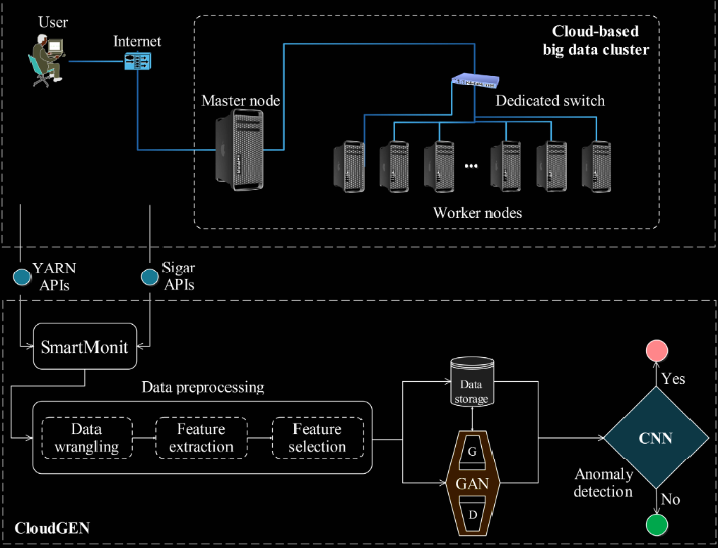
\includegraphics[scale=0.8]{Bilder/CloudGEN.png} Abbildung 1
\\
\\
Die Monitoring-Komponente für die Datenerfassung spielt in CloudGEN eine zentrale Rolle. Sie ist dafür verantwortlich aufkommende Fehlfunktionen oder Leistungsprobleme innerhalb des\\ Big-Data-Systems zu erkennen. Hierbei wird SmartMonit benutzt. SmartMonit ist ein Echtzeit Monitoringsystem für Big Data. Es verfolgt effektiv den Status von Big-Data-Aufgaben und \\ überwacht die Ressourcennutzung in Echtzeit. Es stellt die kontinuierliche Übertragung von \\ Daten von der Quelle in die Zeitreihendatenbank sicher.\nAbsatz Um sämtliche Leistungsmetriken wie die Ausführungszeit, Status, Fortschritt jeder einzelnen Aufgabe sowie Speicherorte der Datenblöcke zu sammeln werden YARN-APIs benutzt. Diese Sammeln diese Metriken vom Masterknoten. Des weiteren werden Metriken zur\\  Ressourcenauslastung wie die CPU Nutzung, Speicherauslastung und Netzwerkverkehr mithilfe von Sigar-Apis erfasst. Die aufgelisteten Metriken werden anschließend an den Consumer \\  übergeben der auf derselben Maschine wie die Datenbank liegt, somit werden die Daten natlos übernommen und in die Datenbank geschrieben. Nachdem alle Daten gesammelt wurden fängt die Datenvorbereitung an, auch Data preprocessing genannt. 
\nAbsatz Die Datenvorbereitung besteht aus drei Schritten. Der erste Schritt ist die Datenbereinigung danach folgt die Merkmalextraktion und zum Schluss eine Merkmalselektion. \\ Die Datenbereinigung auch 'Data Wrangling' genannt dient zur Bereinigung der Daten. \\ Die Rohdaten werden in diesem Schritt umgewandelt und gesäubert, so dass Probleme wie \\ fehlende Werte, Ausreißer und Inkonsistenzen behoben werden und die Integrität des Datensatzes sichergestellt ist. Danach folgt die Merkmalextraktion auch 'Feature Selection' genannt. In diesem Schritt werden aussagekräftige Merkmale extrahiert um relevante Muster für die weitere Analyse zu erfassen und effizient zu nutzen. Der letzte Schritt ist die Merkmalselektion. Dieser Schritt wird auch 'Feature Selection' genannt. Hierbei werden von den Merkmalen aus dem Schritt zuvor die wichtigsten und effektivsten Merkmale in der Entscheidungsphase identifiziert, bevor diese Daten für das Training des GANs benutzt wird. \nAbsatz Die letzte Komponente von CloudGEN ist das Convolutional Neural Network (CNN). Das CNN-basierte Anomalieerkennungssystem ist für die Identifizierung von Anomalien innerhalb des cloudbasierten Big-Data-Systems verantwortlich. Die Implementierung des CNN beginnt mit den vorverarbeiteten Daten, die vom Monitoring-System erzeugt und durch die Komponente \\ Training und Integration generativer Modelle zu Datengenerierung angereichert wurden. \\ Anschließend wird das CNN-Modell auf diesem erweiterten Datensatz trainiert, damit wird sichergestellt dass sowohl reale als auch erzeugte Daten verwendet werden. 
\nAbsatz Zum Schluss möchte ich noch einmal auf die Ergebnisse des Einsatzes von CloudGEN bei der Anomalieerkennung im Bereich eines cloudbasierten Big-Data-Systems eingehen ~\cite{Fallbeispiel}.
\nAbsatz
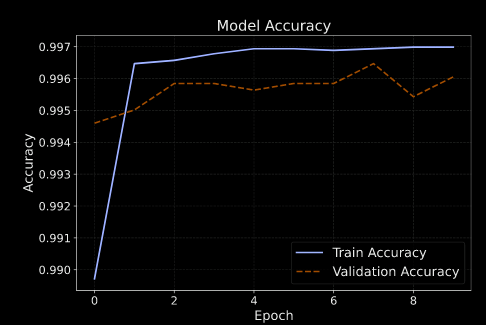
\includegraphics[scale=0.95]{Bilder/ModelAccuracy(9b).png}\\
Abbildung 2
\newpage
\\
Wie im vorhergehenden Diagramm wird dargestellt, wie das Training und die \\ Validierungsgenauigkeit sich über die verschiedenen Epochen entwickelt. Beide Lininen zeigen eine Steigung an, die darauf hinweisen, dass die Genauigkeit konstant ansteigt je mehr Epochen durchlaufen werden. Die Trainingsgenauigkeit scheint sich stetig zu erhöhen und nähert sich \\ nahezu 99,8\%, während die Validierungsgenauigkeit ebenfalls ein ähnliches Muster zeigt, mit leichten Abweichungen ~\cite{Fallbeispiel}.
\nAbsatz
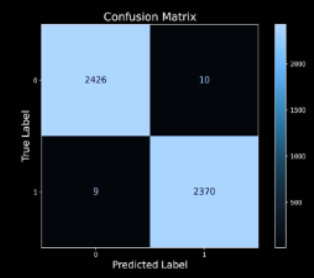
\includegraphics[scale=1.0]{Bilder/Confusion Matrix 10a.png}\\
Abbildung 3
\\
\\
Die Grafik unmittelbar über diesem Textabschnitt zeigt die Leistung des Klassifikationsmodells bei der Unterscheidung zwischen zwei Klassen. Das Modell Klasse 0 bei 2426 Instanzen und Klasse 1 bei 2370 Instanzen korrekt vorhergesagt hat, mit nur 10 falsch-positiven Vorhersagen (Klasse 0 als Klasse 1 vorhergesagt) und 9 falsch-negativen Vorhersagen (Klasse 1 als Klasse 0 vorhergesagt).Die hohe Genauigkeit bei sowohl den wahr positiven und wahr negativen \\ vorhersagen zeigt die Effektivität des Models bei der präzisen Klassifikation der Daten. \\ Des Weiteren möchte ich gerne mit der folgenden Tabelle einen Vergleich der Effektivität im \\ Vergleich zu anderen Modellen zur Anomalieerkennung in Cloud-Computing-Systemen zeigen~\cite{Fallbeispiel}.\\
\\
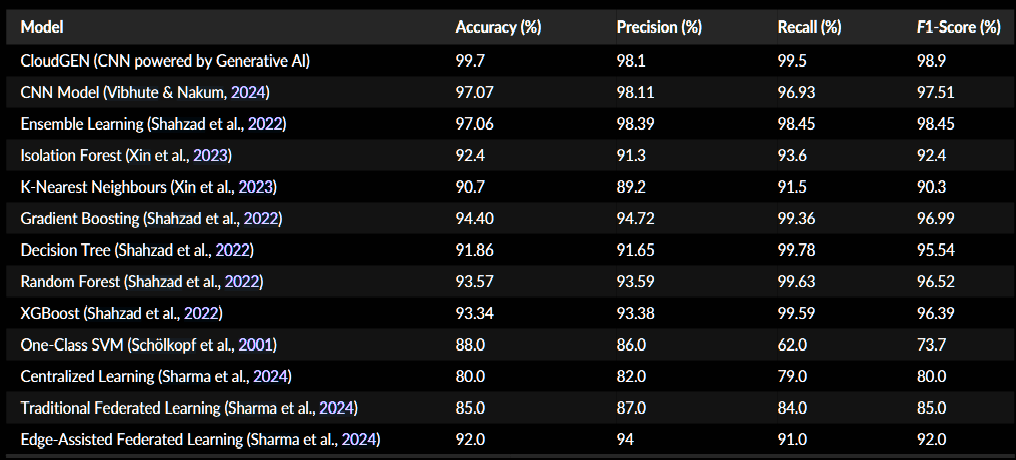
\includegraphics[scale=0.6]{Bilder/ModelleVergleichFallbeispiel table 1.png}\\
Abbildung 4
\\
\\
Diese vergleicht die einzelnen Modelle in den Kategorien: Genauigkeit, Präzision, Recall und dem F1-Score. Unter diesen Kategorien zeigt sich CloudGEN als ein CNN und generatives AI \\ basierendes Modell eine überlegene Leistung in allen Kategorien. Besonders herausragend ist \\ hierbei die Genauigkeit von 99,7\% die noch einmal die Fähigkeit zur Erkennung von \\ Anomalien von CloudGEN zeigt. Durch diese Ergebnisse kann man sehen, dass ein CNN eine effektive Wahl für die Anomalieerkennung in Cloud-Umgebungen ist und die zusätzliche \\ Integration von generativer KI die Leistung noch zusätzlich verbessert. Das zeigt sich vor allem durch die bemerkenswerte Genauigkeit von CloudGEN \cite{Fallbeispiel}.
\nAbsatz
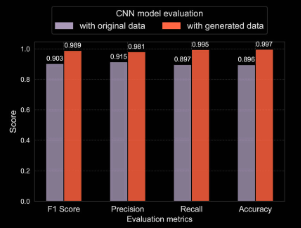
\includegraphics[scale=1.0]{Bilder/Evaluation Matrics 10b.png}\\
Abbildung 5 
\\
\\
In diesem Balkendiagramm werden Bewertungsmetriken wie F1-Score, Präzision, Recall \\ und Genauigkeit für das generative Modell verglichen. Das Modell wird nicht nur auf den \\ Originaldaten evaluiert sondern ebenfalls auf den  generierten Daten. Das auf den generierten \\ Daten bewertete Modell zeigt deutliche Verbesserungen in allen Metriken im Gegensatz zum \\ normalen Modell. Es zeigt sich dass eine Verbesserung von etwa 7\% bis 12\% über alle \\ Kennzahlen besteht. Dies zeigt noch einmal die Wirksamkeit des generativen Modells bei der \\ Verbesserung der Leistungsmetriken des Datensatzes \cite{Fallbeispiel}.
\nAbsatz













\chapter{Vor-/Nachteile und Grenzen}
\label{ch:zsfg}
Als Abschluss meiner Seminararbeit möchte ich einmal auf die Vorteile, Nachteile und die Grenzen der Anomalieerkennung in adaptiven Systemen mit Generativen KI zum heutigen Stand eingehen. Zu Beginn werde ich mit den Vorteilen bei der Nutzung von generativer KI in der \\ Anomalieerkennung schreiben. Ein großer Vorteil von generativer KI bei der Anomalieerkennung ist wie in meinem Fallbeispiel davor erläutert, dass es eine große Verbesserung der Genauigkeit bei der Erkennung von neuen oder auch bereits gelernten Anomalien gibt. Der nächste Vorteil baut auf die verbesserte Genauigkeit auf und beinhaltet eine bessere Anpassungsfähigkeit des Systems das eine generative KI benutzt. Durch das Frühzeitige entdecken neuer oder bekannter Anomalien kann ein adaptives System besser und schneller Anpassungsstrategien entwickeln und umsetzen um einen größeren Schaden entweder komplett zu verhindern oder diesen stark zu minimieren. Ein weiterer Vorteil ist die Analyse und die Entdeckung von Anomalien mit Echtzeit Daten. \\ Da Systeme in der heutigen Zeit immer größer und komplexer werden, gerade mit Hinblick auf Big-Data ist es essenziell eine automatisierte und verlässliche Erkennung von Anomalien in \\ Echtzeit zu unterstützen, da die herkömmlichen statischen Methoden an Ihre Grenzen kommen. Die Datenmengen sind in heutigen Systemen so groß, dass es unmöglich ist Anomalien in Echtzeit vorherzusagen und das System korrekt anzupassen. Durch den Einsatz von generativer KI werden auch Realistische Daten generiert die dem System helfen sich besser flächendeckender \\ vor Fehlern die durch Anomalien entstehen zu schützen. Das System ist robuster gegenüber \\ Neuheiten, da diese eventuell durch das generieren von realistischen Daten bereits zu einem Teil abgedeckt wurden \cite{Fallbeispiel}\cite{Roadmap}. 
\nAbsatz
Weitergehend möchte ich auf die Nachteile eingehen. Ein großer Punkt ist die Ethische \\ Herausforderung für die Systeme. Bereits gelernte Muster können dazu tendieren dinge zu \\ generieren die Menschen aus bestimmten Gruppen diskriminieren. Dabei ist es ebenfalls sehr schwer herauszufinden ob ein Modell bereits Vorurteile gebildet hat und wie es Sie verwendet\cite{Bias}. Damit kommen wir auch bereits zum nächsten Punkt. Die heutigen komplexen Generativen \\ Modelle sind nur schwer nachzuvollziehen. Je größer das Modell ist und je mehr Trainingsdaten verwendet wurden desto schwieriger wird es zu verstehen warum welche Entscheidung \\ getroffen wurde. Durch die Fehlende Transparenz ist man meist gezwungen ein Ergebnis zu \\ akzeptieren wenn es den Erwartungen oder tests entspricht\cite{explainability}. Ein weiteres Problem ist die Prompt Robustheit. Damit ist gemeint dass man einer KI immer wieder den selben Prompt als Eingabe \\ geben kann aber dennoch wird das Ergebnis durch das hinzugefügt Rauschen unterschiedlich sein. Damit ist es schwierig Fehler oder allgemein Outputs zu rekonstruieren\cite{robustness}. Ein letzter Nachteil ist eine Inkorrekte Adaption durch fehlerhafte Daten die zu einem falsches Training des Modells führen. Durch fehlerhafte Adaption des Systems kann es zu Leistungsverschlechterungen \\ kommen die wiederum zu mehr Fehlern im System führen\cite{Adaption}. Auch ein Finanzieller Verlust kann dort zustande kommen. Das folgende Szenario ist selbst ausgedacht um diesen Punkt \\ verständlicher zu machen. In einem Online Shop gibt es einen Sale und viele User besuchen gleichzeitig die Seite. Dabei wäre es Fatal wenn das System seine verfügbaren Ressourcen wie die Kapazität von gleichzeitig verbundenen Usern beschränkt, da es denkt dass ein Angriff folgt, anstatt die Kapazität zu erhöhen. Durch das Drosseln der Kapazität würde es zu finanziellen \\ Verlusten kommen da es einen Anomalie erkennt, obwohl es valide ist. 
\nAbsatz
Zum Schluss meiner Arbeit möchte ich einmal auf die meiner Meinung nach \\ Aktuellen Grenzen eingehen. Ein entscheidender Faktor hierbei wäre das Gleichgewicht zwischen Privatsphäre und Effektivität. Vielen Menschen ist Ihre Privatsphäre sehr wichtig weswegen \\ einige Daten nicht vollständig mit ihrer Zugehörigkeit übermittelt werden dürfen. Hierbei wäre es aber für das Training und die Effektivität des Modells in manchen Fällen sehr hilfreich um bessere und robustere Muster bilden zu können. Jedes Modell ist zudem noch Limitiert durch physische Grenzen. Da dinge wie Rechenleistung, Ressourcen wie Strom oder Geld und Speicherkapazität endlich sind werden Modelle meist durch einen oder mehrere dieser Faktoren begrenzt. Ebenfalls ist eine momentane Grenze die Genauigkeit. Kein Modell hat bislang eine Genauigkeit oder werte in allen Vergleichsmetriken von 100\% . Selbst CloudGEN kommt nur mit 99,8\% nah dran aber erreicht nicht die 100\% . Demnach muss man immer vorsichtig sein, da selbst wenn es nur geringe Lücken sind trotzdem diese gibt. Ein weiterer Punkt hierbei ist noch die Skalierbarkeit. \\ Die heutigen Modelle und Systeme sind sehr groß und natürlich zu einem gewissen teil \\ skalierbar, aber wie bereits erwähnt gibt es auch bei dem skalieren eine physische Grenze. \\ Diese ist an verschiedenen Punkten schneller erreicht als bei anderen. So ist es möglich dass \\ eine große Firma keine Probleme mit den Kosten für den Strom haben wird, aber dafür keinen physischen Platz für die Speicherkapazitäten hat. Zum Schluss würde ich Persönlich sagen dass Generative KI bei der Anomalieerkennung eine wichtige Rolle spielt und zukünftig noch \\ wichtiger wird, aber man immer die Grenzen und nachteile im Auge behalten sollte. Vor allem ist nichts ohne Limit, sei es eine Performance oder auch die Ressourcen. Für die Zukunft wäre es wichtig gerade in der heutigen Zeit auf die knappen aber dennoch verfügbaren Ressourcen die wir haben zu achten und diese effektiv einzusetzen. Dazu sollte man ebenfalls auch noch versuchen die Ergebnisse von den Generativen KIs transparenter zu gestalten, so dass man die  \\Entscheidungen besser nachvollziehen kann. Dennoch ist diese Technologie sehr vielversprechend für unseren bestehenden Systeme und auch wenn sie nicht zu 100\% ausgreift ist, \\ kann sie für zuverlässige Einsätze in der Medizin oder ähnlichen wichtigen Branchen eine große Hilfe werden.    
\nAbsatz
Zusammenfassend lässt sich sagen, dass der Einsatz von generativer KI in vielen Bereich vor allem wenn es um Big-Data geht in der Anomalieerkennung sinn macht und die Performance erheblich verbessert. Dennoch gibt es viele Risiken auf die man Achten muss. Meiner Meinung nach ist dieses Gebiet für die Zukunft sehr wichtig und effizient. Natürlich muss noch definiert werden wo die Privatsphäre des einzelenen anfängt und die Effektivität des Trainings der Modelle aufhört, aber das Potential ist sehr groß. In der Zukunft sollte man sich auf jeden Fall mit der Genauigkeit befassen. Auch wenn es fast unmöglich ist eine 100\% Genauigkeit zu erzielen, kann es trotzdem bei zum Beispiel autonom fahrenden Autos bei einer genauigkeit von 99,9\% und 40 Millionen Autos auf der Straße täglich zu 40.000 Unfällen kommen. Man sollte die Werte mit Vorsicht betrachten und auch wenn sie in einem kleinen Maße sehr vielversprechend klingen sind sie bei einer höheren Skalierung und einem anderen Kontext sehr Kritisch. Ebenfalls sollte man die Erklärbarkeit ein wenig transparenter machen. Durch mehr Transparenz müsste man nicht mehr blind auf die Ergebnisse vertrauen und könnte den Output von Ergebnissen oder auch die Erkennung von Anomalien begründen. Ich denke dass die Benutzung von generativer KI in den nächsten Jahren immer mehr Zuwachs erfahren wird und man sie in unserem Alltag öfter sehen oder mitbekommen wird.    


% Literaturverzeichnis
% Bib-Datei in \Literatur\ba-arbeit.bib 
\bibliography{Literatur/arbeit}
\bibliographystyle{plain}
\addcontentsline{toc}{chapter}{\bibname}


% Algorithmenverzeichnis, falls notwendig. I.d.R. nicht benötigt
%\listof{algorithm}{Algorithmenverzeichnis}
%\addcontentsline{toc}{chapter}{Algorithmenverzeichnis}

% Eidesstattliche Erklaerung

\ihead[Eidesstattliche Erklärung]{}
\chapter*{Eigenständigkeitserklärung}
\label{chapter:erklaerung}
\begin{flushleft}
\normalsize{
\nEinrueck Hiermit versichere ich, dass ich diese Arbeit selbständig verfasst habe. Ich habe keine unzulässige Hilfe Dritter in Anspruch genommen. Zudem habe ich keine anderen als die angegebenen Quellen und Hilfsmittel benutzt und alle Ausführungen (insbesondere Zitate), die anderen Quellen wörtlich oder sinngemäß entnommen wurden, kenntlich gemacht. Die Liste zugelassener Hilfsmittel vom 15.04.2025 ist mir ausdrücklich bekannt.
\nAbsatz
Mir ist bekannt, dass im Falle eines Täuschungsversuches die betreffende Leistung als mit “nicht ausreichend” (5,0) bewertet gilt. Zudem kann ein Täuschungsversuch als Ordnungswidrigkeit mit einer Geldbuße von bis zu 50.000 Euro geahndet werden. Im Falle eines mehrfachen oder sonstigen schwerwiegenden Täuschungsversuchs kann ich zudem exmatrikuliert werden.
\nAbsatz
Mir ist bekannt, dass sich die Prüferin oder der Prüfer bzw. der Prüfungsausschuss zur Feststellung der Täuschung des Einsatzes einer entsprechenden Software oder sonstiger elektronischer Hilfsmittel bedienen kann.
.
\newline\newline\newline\newline
% Unterschriftsbild je nach Bedarf skalieren
% Scale unter 0.5 nicht empfehlenswert; Bilder besser mit Bildbearbeitungsprogrammen wie z.B. GIMP skalieren

\includegraphics[scale=0.5]{Bilder/UnterschriftMeissner.png}
\newline\newline
\balocation, den \today 
}
\end{flushleft}
\addcontentsline{toc}{chapter}{Eigenständigkeitserklärung}

% Ende Dokument
\end{document}